%\VignetteIndexEntry{Bioimagetools}
\documentclass{article}\usepackage[]{graphicx}\usepackage[]{color}
%% maxwidth is the original width if it is less than linewidth
%% otherwise use linewidth (to make sure the graphics do not exceed the margin)
\makeatletter
\def\maxwidth{ %
  \ifdim\Gin@nat@width>\linewidth
    \linewidth
  \else
    \Gin@nat@width
  \fi
}
\makeatother

\definecolor{fgcolor}{rgb}{0.345, 0.345, 0.345}
\newcommand{\hlnum}[1]{\textcolor[rgb]{0.686,0.059,0.569}{#1}}%
\newcommand{\hlstr}[1]{\textcolor[rgb]{0.192,0.494,0.8}{#1}}%
\newcommand{\hlcom}[1]{\textcolor[rgb]{0.678,0.584,0.686}{\textit{#1}}}%
\newcommand{\hlopt}[1]{\textcolor[rgb]{0,0,0}{#1}}%
\newcommand{\hlstd}[1]{\textcolor[rgb]{0.345,0.345,0.345}{#1}}%
\newcommand{\hlkwa}[1]{\textcolor[rgb]{0.161,0.373,0.58}{\textbf{#1}}}%
\newcommand{\hlkwb}[1]{\textcolor[rgb]{0.69,0.353,0.396}{#1}}%
\newcommand{\hlkwc}[1]{\textcolor[rgb]{0.333,0.667,0.333}{#1}}%
\newcommand{\hlkwd}[1]{\textcolor[rgb]{0.737,0.353,0.396}{\textbf{#1}}}%
\let\hlipl\hlkwb

\usepackage{framed}
\makeatletter
\newenvironment{kframe}{%
 \def\at@end@of@kframe{}%
 \ifinner\ifhmode%
  \def\at@end@of@kframe{\end{minipage}}%
  \begin{minipage}{\columnwidth}%
 \fi\fi%
 \def\FrameCommand##1{\hskip\@totalleftmargin \hskip-\fboxsep
 \colorbox{shadecolor}{##1}\hskip-\fboxsep
     % There is no \\@totalrightmargin, so:
     \hskip-\linewidth \hskip-\@totalleftmargin \hskip\columnwidth}%
 \MakeFramed {\advance\hsize-\width
   \@totalleftmargin\z@ \linewidth\hsize
   \@setminipage}}%
 {\par\unskip\endMakeFramed%
 \at@end@of@kframe}
\makeatother

\definecolor{shadecolor}{rgb}{.97, .97, .97}
\definecolor{messagecolor}{rgb}{0, 0, 0}
\definecolor{warningcolor}{rgb}{1, 0, 1}
\definecolor{errorcolor}{rgb}{1, 0, 0}
\newenvironment{knitrout}{}{} % an empty environment to be redefined in TeX

\usepackage{alltt}
\usepackage{authblk}
\IfFileExists{upquote.sty}{\usepackage{upquote}}{}
\begin{document}




\title{Some tools in bioimagetools}
\author[1]{Volker J.~Schmid}
\affil[1]{Bioimaging group, Department of Statistics, LMU Munich}
\maketitle
\tableofcontents
\section{Basis operations: Read and write tiff and bmp.}

\texttt{readTIFF()} and \texttt{writeTIFF()} in the \texttt{tiff} package do not handle 3d stacks the right way. \texttt{bioimagetools} uses \texttt{readTIF()}.
\begin{knitrout}
\definecolor{shadecolor}{rgb}{0.969, 0.969, 0.969}\color{fgcolor}\begin{kframe}
\begin{alltt}
\hlkwd{library}\hlstd{(bioimagetools)}
\end{alltt}


{\ttfamily\noindent\itshape\color{messagecolor}{\#\# Loading required package: EBImage}}

{\ttfamily\noindent\itshape\color{messagecolor}{\#\# Bioimagetools ver.0.3.22}}\begin{alltt}
\hlstd{cell} \hlkwb{<-} \hlkwd{readTIF}\hlstd{(}\hlstr{"http://ex.volkerschmid.de/cell.tif"}\hlstd{)}
\end{alltt}


{\ttfamily\noindent\color{warningcolor}{\#\# Warning in readTIFF(file, all = TRUE, info = TRUE, as.is = as.is, native = native): TIFFReadDirectory: Unknown field with tag 50838 (0xc696) encountered}}

{\ttfamily\noindent\color{warningcolor}{\#\# Warning in readTIFF(file, all = TRUE, info = TRUE, as.is = as.is, native = native): TIFFReadDirectory: Unknown field with tag 50839 (0xc697) encountered}}\begin{alltt}
\hlkwd{print}\hlstd{(}\hlkwd{dim}\hlstd{(cell))}
\end{alltt}
\begin{verbatim}
## [1] 512 512   3  52
\end{verbatim}
\begin{alltt}
\hlkwd{img}\hlstd{(cell,} \hlkwc{z}\hlstd{=}\hlnum{25} \hlstd{,}\hlkwc{col}\hlstd{=}\hlstr{"rgb"}\hlstd{)}
\end{alltt}
\end{kframe}
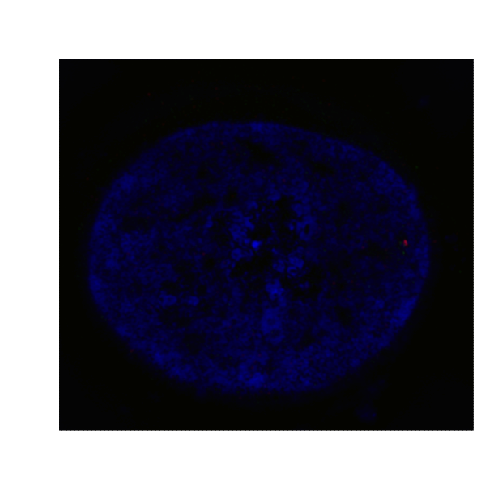
\includegraphics[width=\maxwidth]{figure/unnamed-chunk-2-1} 

\end{knitrout}

\texttt{img()} is a plotting function. It expects a 2d array, unless \texttt{col="rgb"}, which produces a color plot. 
\begin{knitrout}
\definecolor{shadecolor}{rgb}{0.969, 0.969, 0.969}\color{fgcolor}\begin{kframe}
\begin{alltt}
\hlkwd{par}\hlstd{(}\hlkwc{mfrow}\hlstd{=}\hlkwd{c}\hlstd{(}\hlnum{1}\hlstd{,}\hlnum{3}\hlstd{))}
\hlkwd{img}\hlstd{(cell,} \hlkwc{z}\hlstd{=}\hlnum{25}\hlstd{,} \hlkwc{col}\hlstd{=}\hlstr{"r"}\hlstd{)}
\hlkwd{img}\hlstd{(cell,} \hlkwc{z}\hlstd{=}\hlnum{25}\hlstd{,} \hlkwc{col}\hlstd{=}\hlstr{"g"}\hlstd{)}
\hlkwd{img}\hlstd{(cell,} \hlkwc{z}\hlstd{=}\hlnum{25}\hlstd{,} \hlkwc{col}\hlstd{=}\hlstr{"grey"}\hlstd{)}
\end{alltt}
\end{kframe}
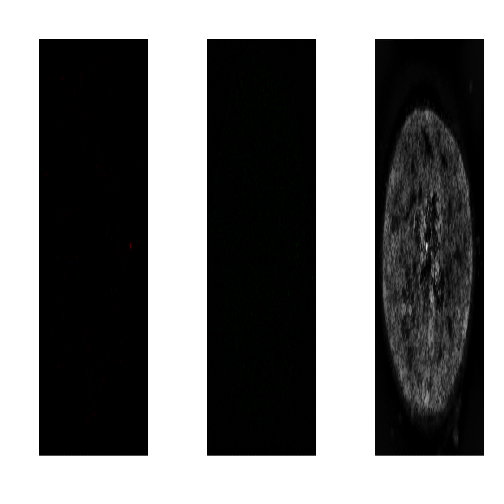
\includegraphics[width=\maxwidth]{figure/unnamed-chunk-3-1} 

\end{knitrout}

\begin{knitrout}
\definecolor{shadecolor}{rgb}{0.969, 0.969, 0.969}\color{fgcolor}\begin{kframe}
\begin{alltt}
\hlkwd{writeTIF}\hlstd{(cell,} \hlkwc{file}\hlstd{=}\hlstr{"my_cell.tif"}\hlstd{)}
\end{alltt}
\begin{verbatim}
## [1] 52
\end{verbatim}
\begin{alltt}
\hlstd{red} \hlkwb{<-} \hlstd{cell[,,}\hlnum{1}\hlstd{,]}
\hlstd{green} \hlkwb{<-} \hlstd{cell[,,}\hlnum{2}\hlstd{,]}
\hlstd{simple} \hlkwb{<-} \hlnum{2}\hlopt{*}\hlstd{EBImage}\hlopt{::}\hlkwd{thresh}\hlstd{(red)}\hlopt{+}\hlstd{EBImage}\hlopt{::}\hlkwd{thresh}\hlstd{(green)}
\hlkwd{writeTIF}\hlstd{(simple,} \hlkwc{file}\hlstd{=}\hlstr{"simple.tif"}\hlstd{)}
\end{alltt}
\begin{verbatim}
## [1] 52
\end{verbatim}
\begin{alltt}
\hlstd{mysimple} \hlkwb{<-} \hlkwd{readClassTIF}\hlstd{(}\hlstr{"simple.tif"}\hlstd{)}
\hlkwd{img}\hlstd{(mysimple[,,}\hlnum{25}\hlstd{],}\hlkwc{col}\hlstd{=}\hlstr{"red"}\hlstd{,}\hlkwc{up}\hlstd{=}\hlnum{3}\hlstd{)}
\end{alltt}
\end{kframe}
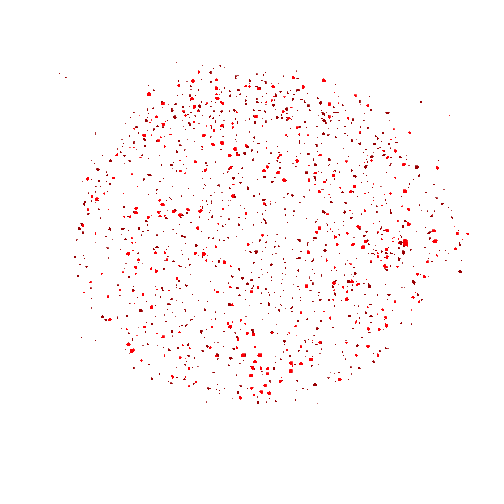
\includegraphics[width=\maxwidth]{figure/unnamed-chunk-4-1} 

\end{knitrout}
\begin{knitrout}
\definecolor{shadecolor}{rgb}{0.969, 0.969, 0.969}\color{fgcolor}\begin{kframe}
\begin{verbatim}
## [1] TRUE
## [1] TRUE
\end{verbatim}
\end{kframe}
\end{knitrout}

Unrelated, Bitmap files can be read
\begin{knitrout}
\definecolor{shadecolor}{rgb}{0.969, 0.969, 0.969}\color{fgcolor}\begin{kframe}
\begin{alltt}
\hlstd{bi}\hlkwb{<-}\hlkwd{readBMP}\hlstd{(}\hlstr{"http://www.statistik.lmu.de/institut/ag/bioimg/bit/ratbert.bmp"}\hlstd{)}
\hlkwd{img}\hlstd{(bi,}\hlkwc{col}\hlstd{=}\hlstr{"greyinvert"}\hlstd{)}
\end{alltt}
\end{kframe}

\includegraphics[width=\maxwidth]{figure/unnamed-chunk-6-1} 

\end{knitrout}

\end{document}
